%*********************************************************************
\subsection{Simulation Experiment}\label{sub:bc_simulation_experiment}
%*********************************************************************

% Introductory paragraph
The application of the Bayesian calibration framework on the \gls[hyper=false]{trace} reflood model parameters against the \gls[hyper=false]{feba} experimental data is based on $6$ different statistical formulations, in the following referred to as \emph{calibration schemes}.
These schemes are distinguished by their respective assumption:
\begin{itemize}
	\item \texttt{w/ Bias, All}. The first calibration scheme assumes that the \gls[hyper=false]{trace} model is an imperfect simulator of the reflood phenomena in the the \gls[hyper=false]{feba} experiment.
		As such it considers a model bias term (as described furter below) in the calibration process. Furthermore, in this scheme, all available types of experimental data are considered.
		The data includes the clad temperature at different time points and at different axial locations (will be succinctly referred to below as the $TC$ output or data),
		the pressure drop at different time points and at different axial segments (referred to as the $DP$ output or data),
		and the collected liquid carryover at different time points (referred to as the $CO$ output or data).
		As mentioned, following the results of the previous chapter, only the most influential $8$ reflood model parameters are considered for the calibration. 
	\item \texttt{w/ Bias, TC}, \texttt{w/ Bias, DP}, and \texttt{w/ Bias, CO} are three variants of the scheme \texttt{w/ Bias, All} in which only one type of experimental data (respectively, output) is considered at a time for the calibration.
		The purpose of these schemes is to investigate the effect of using different types of data from the same experiment to constrain the model parameters prior uncertainties.
		The calibration is still conducted for the $8$ reflood model parameters and by considering the model bias term.
	\item \texttt{w/o Bias} is conducted to provide a comparison with the calibration. This scheme is similar to the scheme \texttt{w/ Bias, All};
		it uses all available types of experimental data to calibrate the $8$ reflood model parameters, except that no model bias term is included in the formulation.
		In essence, this scheme assumes that the \gls[hyper=false]{trace} model perfectly describes the reflood phenomena in the \gls[hyper=false]{feba} experiment.
	\item \texttt{w/ Bias, no dffbVIHT}. The last calibration scheme is conducted as to investigate the effect of excluding, from the calibration process, an influential parameter (\texttt{dffbVIHT}) that is later found from the scheme \texttt{w/ Bias, All} to be strongly correlated.
		Except for calibrating only $7$ reflood model parameters, this scheme used similar assumptions as the first scheme.
\end{itemize}

The six calibration schemes above aim to update the prior uncertainties of the model parameters using the available experimental data from \gls[hyper=false]{feba} test No. 216.
The six posterior \gls[hyper=false]{pdf} formulation are then directly sampled using an ensemble \gls[hyper=false]{mcmc} sampler to obtain six different sets of posterior samples.
To avoid an excessive computational cost of having to run \gls[hyper=false]{trace} hundreds thousands of times (if not more), the \gls[hyper=false]{gp} metamodel for the \gls[hyper=false]{trace} model developed in Chapter~\ref{ch:gp_metamodel} is used to substitute \gls[hyper=false]{trace} run.

These different sets of samples are then analyzed to assess the effect of using different calibration schemes in constraining the prior uncertainties of the model parameters. 
Finally, the resulting posterior samples from different schemes are used in forward \gls[hyper=false]{uq} on the \gls[hyper=false]{trace} model of different \gls[hyper=false]{feba} tests (corresponding to different boundary conditions, namely system pressure and reflood rate).
This final exercise is aimed to assess the implication of the posterior uncertainties from different calibration schemes on (and their applicability for) the prediction under conditions different from the condition of the calibration data.

Each calibration scheme, the \gls[hyper=false]{mcmc} sampler, and a method to evaluate the posterior prediction uncertainty wil be detailed further below. 

%-------------------------------------------------------------------------------------------
\subsubsection{Experimental Data and Observation Layout}\label{subsub:bc_observation_layout}
%-------------------------------------------------------------------------------------------

%--------------------------------------------------------------------------------------------
\subsubsection{Gaussian Process Approximation for TRACE Simulation}\label{subsub:bc_gp_trace}
%--------------------------------------------------------------------------------------------

%-----------------------------------------------------------------------
\subsubsection{Modeling the Model Bias Term}\label{subsub:bc_model_bias}
%-----------------------------------------------------------------------

%-----------------------------------------------------------------------
\subsubsection{Calibration Schemes}\label{subsub:bc_calibration schemes}
%-----------------------------------------------------------------------

% Summary
Table~\ref{tab:ch5_calibration_schemes} summarizes the different calibration schemes considered in this study.
\begin{table*}[!htbp]\centering
\ra{0.9}
\begin{adjustwidth*}{}{-3cm}
\caption{Bayesian calibration schemes conducted for the \gls[hyper=false]{trace} reflood model parameters against data from \gls[hyper=false]{feba} test No. $216$.}
\label{tab:ch5_calibration_schemes}
\begin{tabular}{@{}clccccrc@{}}\toprule
\multirow{2}{*}{No.} & \multirow{2}{*}{\shortstack[c]{Calibration Scheme}} 	& \multirow{2}{*}{\shortstack[c]{Model Bias\\Term}}	& \multicolumn{3}{c}{Types of Output} & \phantom{a} & \multirow{2}{*}{\shortstack[c]{Reflood Model\\Parameters \footnotesize{(total number)}}} \\
																															  \cmidrule{4-6}
    &                                 					& 						& $TC$				& $DP$     		& $CO$   				&&	\\ \midrule
1   & \texttt{w/ Bias, All}											& \Checkmark  & \Checkmark  & \Checkmark  & \Checkmark  	&& All \footnotesize{($8$)}          				\\
2   & \texttt{w/ Bias, TC}     									& \Checkmark  & \Checkmark	&							&          			&& All \footnotesize{($8$)}           			\\
3   & \texttt{w/ Bias, DP}     									& \Checkmark 	&         		& \Checkmark	&								&& All \footnotesize{($8$)} 								\\
4   & \texttt{w/ Bias, CO}       								& \Checkmark 	& 						& 						& \Checkmark		&& All \footnotesize{($8$)}           			\\
5   & \texttt{w/o Bias}               					&          		& \Checkmark  & \Checkmark  & \Checkmark		&& All \footnotesize{($8$)}	          			\\
6   & \texttt{w/ Bias, no dffbVIHT}             & \Checkmark  & \Checkmark  & \Checkmark  & \Checkmark		&& Excluding \texttt{dffbVIHT} \footnotesize{(7)}\\
\bottomrule
\end{tabular}
\end{adjustwidth*}
\end{table*}

%---------------------------------------------------------------------------------------
\subsubsection{MCMC Simulation using Ensemble Sampler}\label{subsub:bc_calibration_mcmc}
%---------------------------------------------------------------------------------------

%-----------------------------------------------------------------------------------------
\subsubsection{Evaluating Calibration Results}\label{subsub:bc_calibration_evaluation}
%-----------------------------------------------------------------------------------------


% The statistical calibration framework revisited

% Observation Layout

% Modeling the simulator output

% Modeling the discrepancy

% Likelihood Formulation

% 

% 

% 

% Analyzing convergence
\clearpage
\begin{sidewaysfigure}
	\centering
	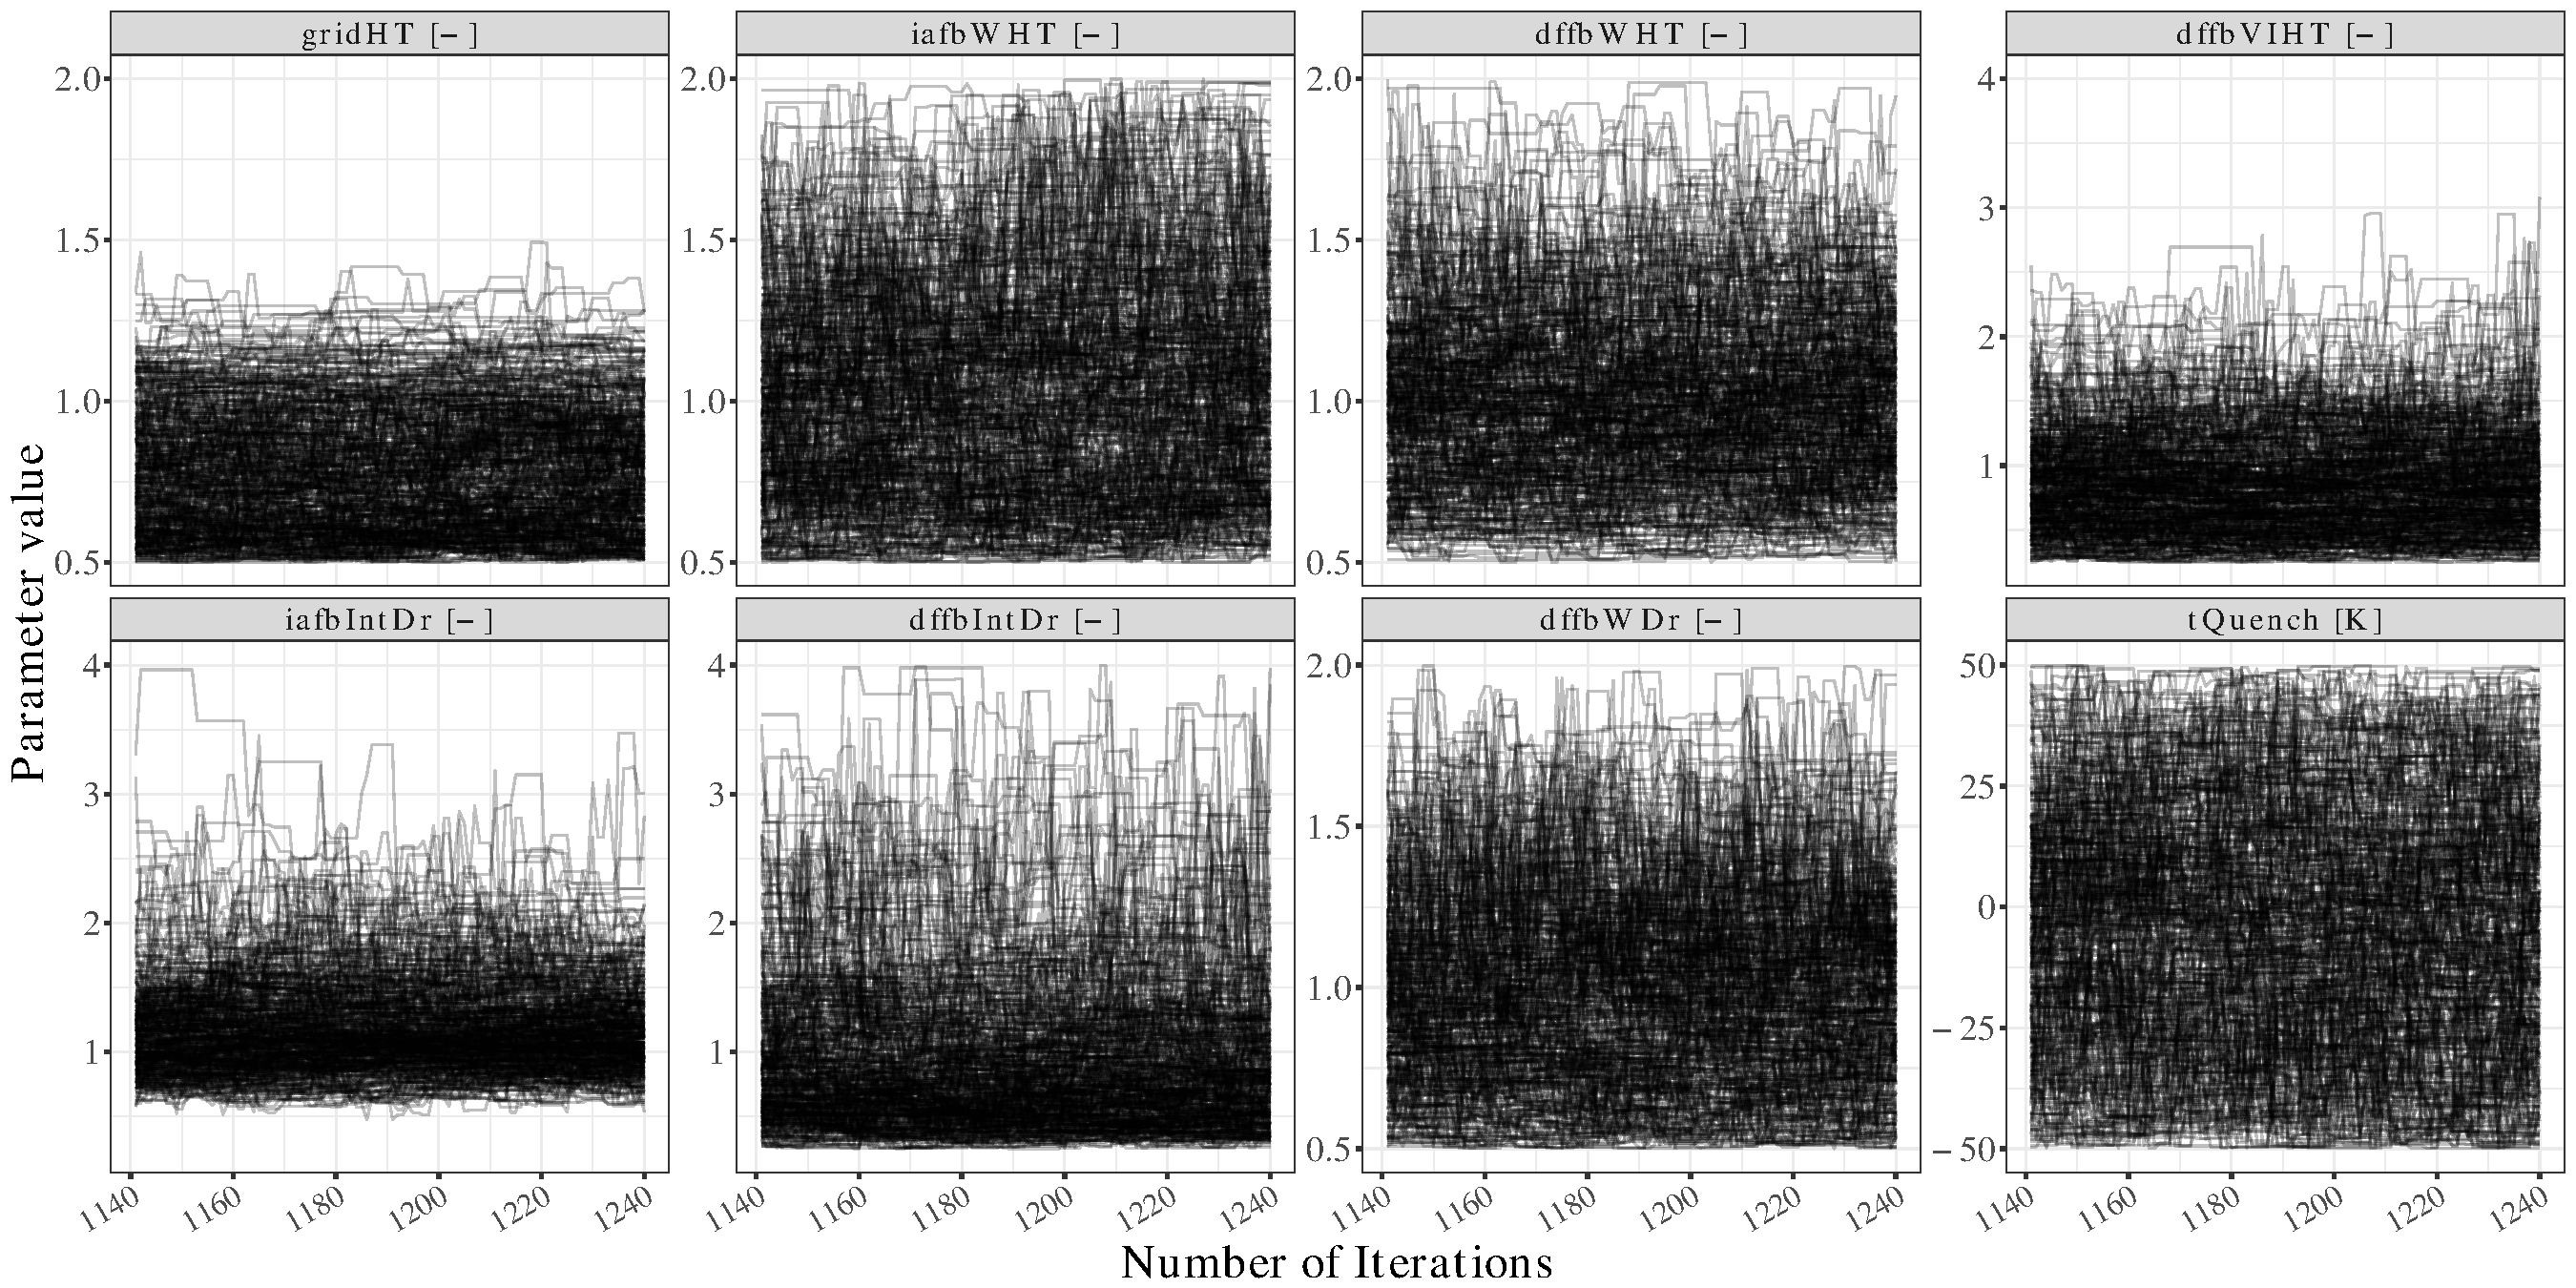
\includegraphics[width=0.90\textwidth]{../figures/chapter5/figures/plotEnsTraceDiscAllCentered}
		\captionof{figure}[Ensemble trace plots for each model parameter of calibration with model bias term.]{Ensemble trace plots for each model parameter of calibration with model bias term. Shown here is for the last $100$ iterations (out of $1'240$ post-burn-in iterations) and for $400$ walkers (out of $1'000$ walkers).}
	\label{fig:ch5_plot_ens_trace_all_disc_centered}
\end{sidewaysfigure}
\clearpage